\section{\large \textcolor{blue}{As leis da Termodinâmica}}

\begin{flushleft}
\textbf{\textcolor{blue}{\Large Quest\~ao - IFSP 2015 - Lei de Fourier da Condu\c{c}\~ao de Calor}}\\
\noindent

\subsection{Quest\~ao IFSP 2015 - Lei de Fourier da Condu\c{c}\~ao de Calor}

Em um experimento sobre condutividade térmica dos metais, uma barra metálica homogênea e de área de secção transversal uniforme, isolada termicamente do meio externo, foi colocada entre duas fontes a temperaturas diferentes ($T_A$ e $T_B$). Dois termômetros foram colocados de forma a medirem a temperatura da barra em dois pontos diferentes e estabilizaram seus valores naqueles mostrados na figura abaixo.

\vspace{0.3cm}

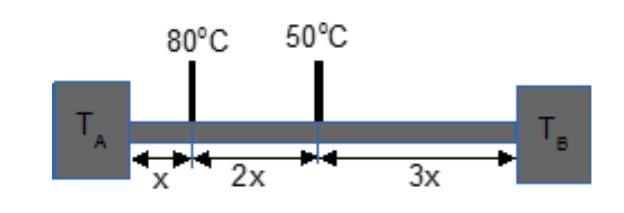
\includegraphics[width=0.8\textwidth]{figures/barra_termica.png}

\vspace{0.3cm}

A temperatura das fontes ($T_A$ e $T_B$) são, respectivamente:

\begin{itemize}
\item[(A)] 90\textdegree C e 20\textdegree C
\item[(B)] 125\textdegree C e 5\textdegree C
\item[(C)] 120\textdegree C e 16,6\textdegree C
\item[(D)] 95\textdegree C e 5\textdegree C
\item[(E)] 20\textdegree C e 90\textdegree C
\end{itemize}

\vspace{0.5cm}

\textcolor{red}{\textbf{Solução:}}\\

Como a barra é homogênea, de área constante e está isolada termicamente, o sistema está em equilíbrio térmico e o fluxo de calor é constante. A distribuição de temperatura é linear em cada trecho. Assim, podemos aplicar a relação:

\[
\frac{\Delta T_1}{L_1} = \frac{\Delta T_2}{L_2} = \frac{\Delta T_3}{L_3}
\]

Dividindo a barra em 3 trechos:
\begin{itemize}
\item Do ponto $T_A$ até 80\textdegree C: comprimento $x$, variação de temperatura: $T_A - 80$
\item De 80\textdegree C até 50\textdegree C: comprimento $2x$, variação de temperatura: $30$
\item De 50\textdegree C até $T_B$: comprimento $3x$, variação de temperatura: $50 - T_B$
\end{itemize}

Igualando as razões:

\[
\frac{T_A - 80}{x} = \frac{30}{2x} \Rightarrow T_A - 80 = 15 \Rightarrow T_A = 95^\circ \text{C}
\]

\[
\frac{30}{2x} = \frac{50 - T_B}{3x} \Rightarrow 15 = \frac{50 - T_B}{3} \Rightarrow 50 - T_B = 45 \Rightarrow T_B = 5^\circ \text{C}
\]

\vspace{0.3cm}

A resposta correta é a alternativa \colorbox{green!50}{\textbf{(D)}}.

\end{flushleft}


\begin{flushleft}
\textbf{\textcolor{blue}{\Large Quest\~ao - }}\\
\noindent

\subsection{Quest\~ao }

\begin{itemize}
\item[(A)] 
\item[(B)] 
\item[(C)]
\item[(D)] 
\item[(E)] 
\end{itemize}

\vspace{0.5cm}

\textcolor{red}{\textbf{Solução:}}\\


A resposta correta é alternativa \colorbox{green!50}{\textbf{...}}.

\end{flushleft}

\noindent\rule{\linewidth}{0.6pt}\\
